\section{Тестирование и разработка алгоритмов компьютерного зрения на изображении и видео}
\subsection{Эксперимент}
Цель эксперимента состояла в том, чтобы проверить эффективность работы алгоритмов, методов компьютерного зрения в антропометрии, проверить обоснованность конструкции системы, учитывая влияние внешних факторов на точность алгоритма.

Система компьютерного зрения в антропометрии состоит из 3 основных частей: извлечение антропометрических признаков, классификация антропометрических признаков и применения их на практике. 

Процесс извлечения  антропометрических признаков выполняется следующим образом. Во-первых, происходит обнаружение и распознавание объектов методами вычитания фона и обнаружения лица человека. Следующим шагом является сегментация и определение ключевых точек с помощью метода разреза на графах (Graph cuts) и итеративного алгоритма ближайших точек (Iterative Closest Point - ICP). Процесс классификации антропометрических признаков состоит из двух частей: обучение и тестирование. Важным шагом в этом процессе является  создание учебной модели для классификации новых данных с высокой точностью. 

В данной работе рассматривается построение приложения компьютерного зрения в антропометрии для двух областей: пошив одежды и фитнес-тестирование. В этом разделе рассматривается возможность создания 3D-моделей, классифиции размеров человеческого тела, способность анализировать антропометрические данные в соответствии со стандартом IBM, Fitness и т.д. Также, сравнивается наш метод и алгоритм построения системы компьютерного зрения антропометрии и другие алгоритмы, чтобы найти подходящий для успешной реализации.

\subsection{Тестирование разработанного ПО – извлечение и классификация антропометрических признаков на видео}
Эксперимент проводился на основе языка C ++ (Visual Studio 2010), Java, Matlab с использованием открытой библиотеки компьютерного зрения - OpenCV, библиотеки моделирования 3D для компьютеров и смартфонов - Min3D и библиотеки дизайн 3D моделей - Humanmaker. 

\textbf{Оборудование тестирования:}

\begin{itemize}
	\item Ноутбук с процессором Intel Core 2 Duo (2.3 ГГц), 3 Гб оперативной памяти, камера 1,3 мегапикселей, которая передает 30 кадров в секунду с разрешением  $320 * 240$ пикселей;
	\item Смартфон Самсунг с фронтальной камерой 5 мегапикселей.

\end{itemize}
Эксперимент проводился на основе данных, собранных с помощью личного устройства. На этапе сбора данных пользователь стоит перед фронтальной камерой телефона (расстояние такое, чтобы тело полностью было в кадре), выполняется серия движений, поворот на 90 градусов налево, направо и наоборот. Первоначально будут собираться данные с изображения. Приложение идентифицирует объект, который появляется в кадре и определяет, человек это или нет (на основе обнаружения лица). Затем программа автоматически собирает и выполняет вычитание фона изображения, сегментацию частей человеческого тела, определяет ключевые точки на теле. Происходит калибровка для расчета антропометрических признаков.

Для проверки правильности работы программы, эксперименты проводились несколько раз для одного и того же объекта, в разном времени и месте, в различных условиях шума и освещения, таких как, эксперименты \ref{img29}.

\begin{figure}[ht!]
\centering
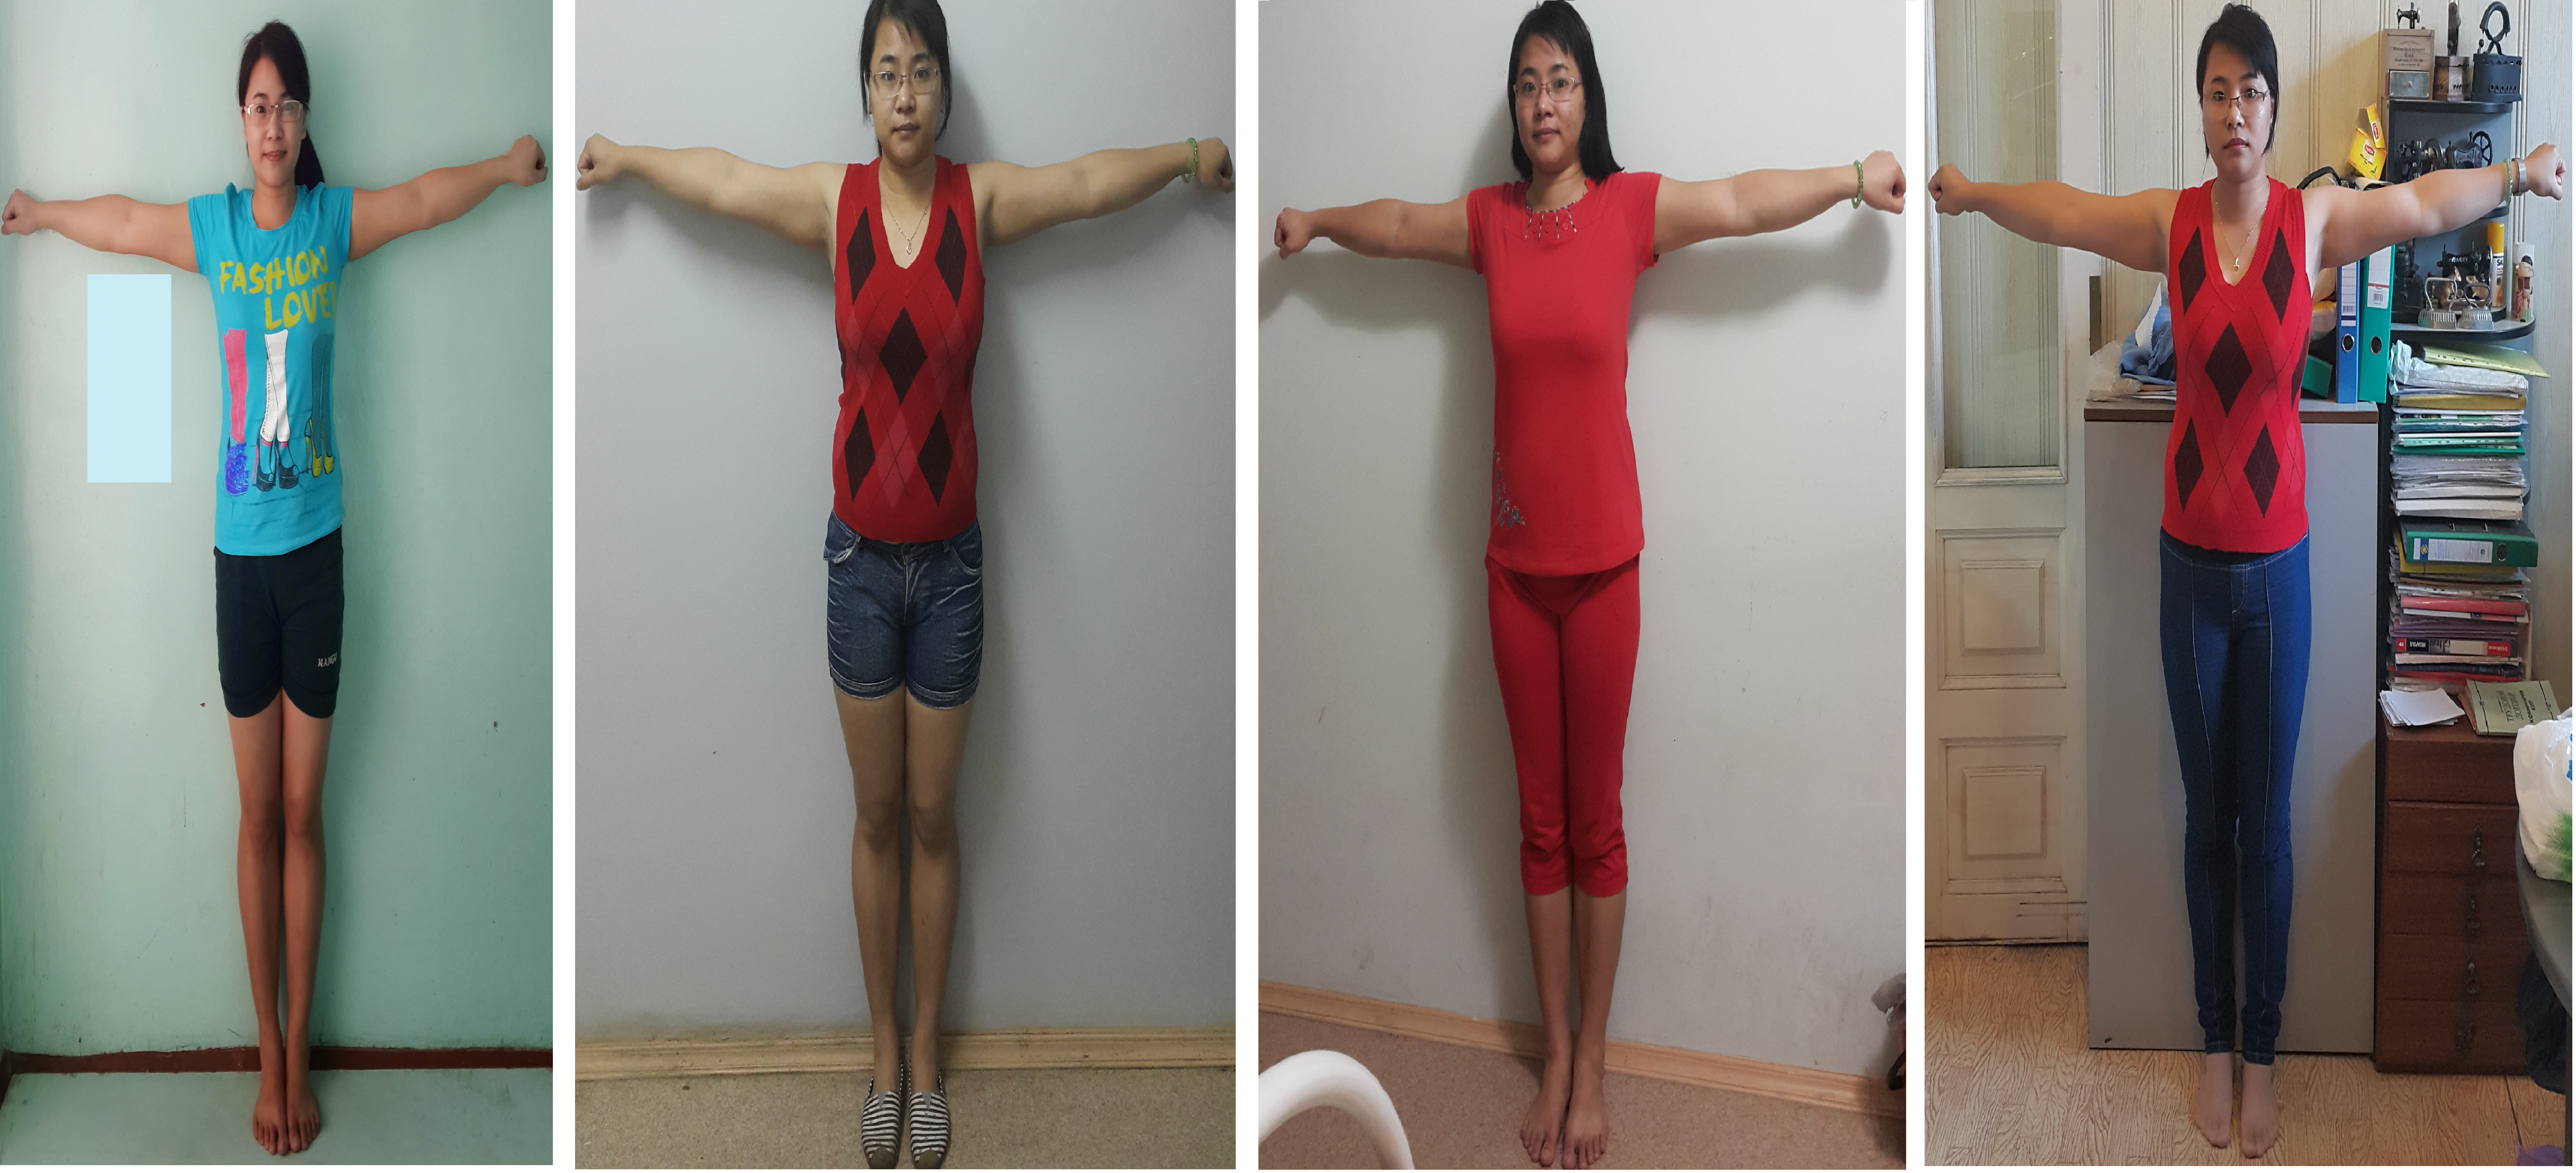
\includegraphics [scale=0.1] {images/h29.png}
\begin{center}
%\captionsetup{justification=justified, labelsep=period}
\caption{Пример данных эксперимента.} \label{img29}
\end{center}
\end{figure}

База данных для экспериментов на компьютере состоит из 6 видео. Эта база данных была создана, чтобы получить данные для тестирования и оценки эффективности работы методов и алгоритмов компьютерного зрения на видео. Создание этой базы необходимо, чтобы учитывать влияние различных факторов на производительность системы (\ref{img36}), (\ref{img37}).

\begin{figure}[ht!]
\centering
\includegraphics [scale=0.5] {images/h36.png}
\begin{center}
%\captionsetup{justification=justified, labelsep=period}
\caption{Результаты извлечения антропометрических признаков и 3D-моделей для женщин.} \label{img36}
\end{center}
\end{figure}
\begin{figure}[ht!]
\centering
\includegraphics [scale=0.5] {images/h37.png}
\begin{center}
%\captionsetup{justification=justified, labelsep=period}
\caption{Результаты извлечения антропометрических признаков и 3D-моделей для мужчин.} \label{img37}
\end{center}
\end{figure}

В ходе эксперимента были использованы алгоритмы компьютерного зрения и извлечения антропометрических признаков. Для этого используются алгоритмы разреза на графах, а также итеративные алгоритмы ближайших точек двух видов: из 24 ключевых точек и 28 ключевых точек для сравнения результата алгоритма вычитания фона и метода выпуклой оболочки \ref{tab7} . В нашей работе \cite{long1} изложен метод измерения различных антропометрических признаков на основе анализа цифровых изображений. Для более эффективного измерения признаков предлагается использовать субпиксельную обработку и анализ выпуклой оболочки. В нашем подходе контур тела описывается выпуклостью дефектов треугольников. Тела представлены треугольниками. Такие треугольники имеют три координаты: выпуклый дефект старт, выпуклый дефект конец, и выпуклый дефект положения точек, соответственно помечены. Мы определили области интересов, которые содержат части тела. Таким образом, мы получили 5 выпуклых областей с соответствующими условиями.

\begin{table}[b!]%
\begin{center}
\caption{Результаты извлечения антропометрических признаков}\label{tab7}
\begin{tabular}{ |c|c|c|c| } 
\hline
  \multirow{3}{*}& Graph-cuts + ICP  & Graph-cuts + ICP  &Вычитание фона \\
								 & (28 ключевых - &(24 ключевых - & + выпуклая\\
	               & - точек)       & - точек)      & оболочка\\
\hline
\multirow{2}{*}{Груди} & \multicolumn{3}{|c|}{93}\\ 
                         & 92.85 & 90.75&85.0 \\ 
\hline
\multirow{2}{*}{Талия} & \multicolumn{3}{|c|}{75}\\ 
                         & 74.80 & 72.0 & 69.79 \\ 	
\hline
\multirow{2}{*}{Бедра} & \multicolumn{3}{|c|}{91}\\ 
                         & 91.3 & 89.65 & 88.65 \\ 
\hline
\multirow{2}{*}{Длина рук} & \multicolumn{3}{|c|}{50}\\ 
                         & 50.40 & 47.62 & 40.30 \\
\hline
\multirow{2}{*}{Обхват } & \multicolumn{3}{|c|}{29}\\ 
                бицепса  & 28.50 & 27.31 & 32.50\\
\hline
\multirow{2}{*}{Обхват } & \multicolumn{3}{|c|}{36}\\ 
                 шеи        & 36.21 & 35.70 & 38.95\\	
\hline
\multirow{2}{*}{Длина } & \multicolumn{3}{|c|}{40}\\ 
                 спины        & 40.10 & 38.75 & 56.50\\	
\hline
\multirow{2}{*}{Ширина } & \multicolumn{3}{|c|}{36}\\ 
                  плеча       & 36.25 & 34.30 & 31.90\\
\hline
\multirow{2}{*}{Длина } & \multicolumn{3}{|c|}{13}\\ 
                 плеча        & 13.10 & 12.83 & 15.56\\
\hline
\end{tabular}
\end{center}
\end{table}%\vspace{10mm}

В (рис. \ref{img24}) описан результат эксперимента проверки точности извлечения антропометрических признаков 3 методов (разреза на графах + ICP для 28 опорных точек, разреза на графах + ICP для 24 опорных точек, вычитание фона + выпуклая оболочка) с ручной метода для одного человека.

\begin{figure}[ht!]
\centering
\includegraphics [scale=0.8] {images/h24.png}
\begin{center}
%\captionsetup{justification=justified, labelsep=period}
\caption{Сравнение результата эксперимента.} \label{img24} \label{img24}
\end{center}
\end{figure}
